\chapter{Implementation}
\label{chapter:implementation}

The following Sections describe an implementation of the proposed method
described in Chapter \ref{chapter:proposed-method}.

\section{Defining the Input Dataset}
\label{section:defining-the-input-dataset}

The dataset to be used must consist of a time series that represent the prices
of a financial market. The number of data points needs to be greater than the
number of data points to be used for the preprocessing algorithm (see Section
\ref{section:preprocessing-a-financial-market-using-retracements:implementation}). To
better understand this, consider the scenario where 100 data points are used to
generate the sets of retracements for the price at time $t_0$: none of the first
100 prices in the dataset are useful for the proposed method, as no retracements
can yet be calculated and associated to them due to lack of data. Once the first
100 data points are used to generate the sets of retracements, one can associate
them to the 101st price in the time series.

Although it is common in financial market datasets to provide the open, high,
low and close prices of each of the data points, this implementation of the
proposed method only uses the close price of each session. For example, in a
dataset consisting of 1 hour sessions, the highest and lowest price achieved in
that hour, and the opening price are discarded, and only the last price recorded
in that hour is used. It is also common to see a volume count in the datasets;
this information is also discarded. Finally, the time associated to each session
in the dataset is used, which means that from any financial market dataset used,
this implementation only uses the close price of each session and the time at
which this close price occurred.

\section{Preprocessing a Financial Market using Retracements}
\label{section:preprocessing-a-financial-market-using-retracements:implementation}

After a trial and error process in undocumented initial experiments, it was
found convenient to use 20 data points to generate the sets of retracements
associated to each price point. The subjective metrics used to determine this
are the processing time required and the interpretability of the plots generated
with this parameter. The author of this thesis used the resulting plots as a
guideline to perform a series of successful real trades in multiple foreign
exchange markets.

The ratios used to calculate the retracements are determined by the beliefs of
the agent preprocessing the raw market data. These ratios are represented by a
vector of a size that can vary from 1 to 6 random real numbers. These random
real numbers have a value that lies in the interval $[0, 2]$. The vector
representing the beliefs varies in size in order to increase the method's
capacity of representing different agent profiles. The size limit of 6 beliefs
was determined arbitrarily.

After calculating the sets of retracements for the last 20 price differences,
these are used to determine weighed price areas. The price areas are intervals
of prices of a fixed height, which is 10 asset units in the case of this
implementation. For example, in the case of the Euro vs United States Dollar,
the price interval $[1.1300, 1.1400]$ can be divided into ten price areas of 10
units each, as a single unit in this market is equivalent to $0.0010$. If three
retracement prices are contained in the interval $[1.1300, 1.1310\right)$, then
this area is associated a weight of $3$. An example of such price areas is
shown in Figure \ref{figure:example-of-retracement-areas}. The heatmap scale
is shown at the right, showing that blocks with a greater weight are of a
lighter color, while blocks with a lower weight are of a darker color.

\begin{figure}
\caption{Example of retracement areas} \centering
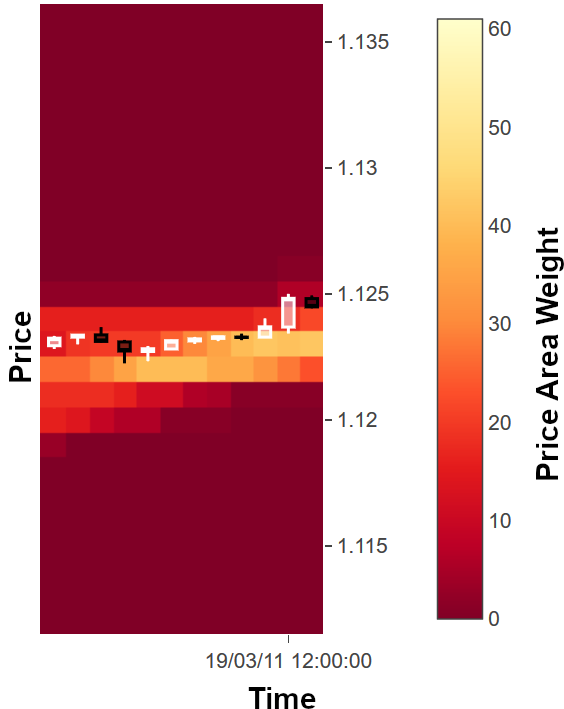
\includegraphics[width=1.0\textwidth]{img/retracement-areas.png}
\label{figure:example-of-retracement-areas}
\end{figure}

\section{Using Agents to Represent Traders in a Financial Market}
\label{section:using-agents-to-represent-traders-in-a-financial-market:implementation}

An agent is represented by a vector containing its beliefs and by a matrix
containing its rules. The elements in the belief vector, as mentioned in
\ref{section:defining-the-input-dataset}, are random real numbers with values in
the interval $[0, 2]$. In the case of the rules, the elements are vectors of
three elements, where the first and second elements are real numbers, with
random values in the interval $[0, 100]$, which represent the means of Gaussian
membership and non-membership functions, respectively. The last element
represents the indeterminacy in the intuitionistic fuzzy set determined by the
membership and non-membership functions. This indeterminacy is a random real
number, which takes a value in the interval $[0, 1]$, influences both the
membership and non-membership in the following way: if the indeterminacy is
equal to $\pi$, then the max membership value in the membership function is
equal to $1 - \pi$, and the max non-membership value in the non-membership
function is equal to $\pi$.

\section{Representing the Agents' Rules as Intuitionistic Fuzzy Systems}
\label{section:representing-the-agents-rules-as-intuitionistic-fuzzy-systems}

\section{Generating the Agent-Based Model}
\label{section:generating-the-agent-based-model}

\section{Extracting Insights about a Financial Market}
\label{section:extracting-insights-about-a-financial-market}
